\documentclass[tikz]{standalone}
\usepackage{pgfplots}
\pgfplotsset{compat=1.15}
\usepackage{mathrsfs}
\usetikzlibrary{arrows,calc}
\usepackage{tkz-euclide}

\pagestyle{empty}

\definecolor{AngleClr}{rgb}{0,0.39215686274509803,0}
\definecolor{ShapeClr}{rgb}{0.6,0.2,0}

\begin{document}

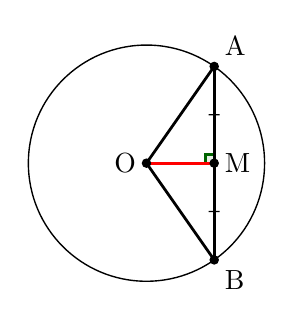
\begin{tikzpicture}[scale=.75]
\tkzSetUpLine[line width=1pt,color=black]
\tkzSetUpPoint[fill=black]

\tkzDefPoints{0/0/O,2/0/X}

\tkzDefPoint(-55:2){B}
\tkzDefPoint(55:2){A}

\tkzDefPointBy[projection=onto A--B](O)\tkzGetPoint{M}

\tkzDrawCircle[draw=black,fill=white,line width=0.5pt](O,X)

\tkzMarkRightAngle[line width=1pt, size=.15,color=AngleClr,fill=AngleClr,fill opacity=0.1](O,M,A)

\tkzDrawSegments[line width=1pt,color=black](O,A O,B A,B)
\tkzDrawSegments[line width=1pt,color=red](O,M)



\tkzDrawPoints[size=3](A,B,O,M)

\tkzLabelPoint[above right](A){$\rm A$}
\tkzLabelPoint[below right](B){$\rm B$}
\tkzLabelPoint[right](M){$\rm M$}
\tkzLabelPoint[left](O){$\rm O$}

\tkzMarkSegments[mark=|,size=2](M,A M,B)

\end{tikzpicture}
\end{document}
